%File: formatting-instructions-latex-2024.tex
%release 2024.0
\documentclass[letterpaper]{article} % DO NOT CHANGE THIS
\usepackage{aaai24}  % DO NOT CHANGE THIS
\usepackage{times}  % DO NOT CHANGE THIS
\usepackage{helvet}  % DO NOT CHANGE THIS
\usepackage{courier}  % DO NOT CHANGE THIS
\usepackage[hyphens]{url}  % DO NOT CHANGE THIS
\usepackage{graphicx} % DO NOT CHANGE THIS
\urlstyle{rm} % DO NOT CHANGE THIS
\def\UrlFont{\rm}  % DO NOT CHANGE THIS
\usepackage{natbib}  % DO NOT CHANGE THIS AND DO NOT ADD ANY OPTIONS TO IT
\usepackage{caption} % DO NOT CHANGE THIS AND DO NOT ADD ANY OPTIONS TO IT
\frenchspacing  % DO NOT CHANGE THIS
\setlength{\pdfpagewidth}{8.5in}  % DO NOT CHANGE THIS
\setlength{\pdfpageheight}{11in}  % DO NOT CHANGE THIS
%
% These are recommended to typeset algorithms but not required. See the subsubsection on algorithms. Remove them if you don't have algorithms in your paper.
\usepackage{algorithm}
\usepackage{algorithmic}
\usepackage{booktabs}


%
% These are are recommended to typeset listings but not required. See the subsubsection on listing. Remove this block if you don't have listings in your paper.
\usepackage{newfloat}
\usepackage{listings}
\DeclareCaptionStyle{ruled}{labelfont=normalfont,labelsep=colon,strut=off} % DO NOT CHANGE THIS
\lstset{%
	basicstyle={\footnotesize\ttfamily},% footnotesize acceptable for monospace
	numbers=left,numberstyle=\footnotesize,xleftmargin=2em,% show line numbers, remove this entire line if you don't want the numbers.
	aboveskip=0pt,belowskip=0pt,%
	showstringspaces=false,tabsize=2,breaklines=true}
\floatstyle{ruled}
\newfloat{listing}{tb}{lst}{}
\floatname{listing}{Listing}
%
% Keep the \pdfinfo as shown here. There's no need
% for you to add the /Title and /Author tags.
\pdfinfo{
/TemplateVersion (2024.1)
}

% DISALLOWED PACKAGES
% \usepackage{authblk} -- This package is specifically forbidden
% \usepackage{balance} -- This package is specifically forbidden
% \usepackage{color (if used in text)
% \usepackage{CJK} -- This package is specifically forbidden
% \usepackage{float} -- This package is specifically forbidden
% \usepackage{flushend} -- This package is specifically forbidden
% \usepackage{fontenc} -- This package is specifically forbidden
% \usepackage{fullpage} -- This package is specifically forbidden
% \usepackage{geometry} -- This package is specifically forbidden
% \usepackage{grffile} -- This package is specifically forbidden
% \usepackage{hyperref} -- This package is specifically forbidden
% \usepackage{navigator} -- This package is specifically forbidden
% (or any other package that embeds links such as navigator or hyperref)
% \indentfirst} -- This package is specifically forbidden
% \layout} -- This package is specifically forbidden
% \multicol} -- This package is specifically forbidden
% \nameref} -- This package is specifically forbidden
% \usepackage{savetrees} -- This package is specifically forbidden
% \usepackage{setspace} -- This package is specifically forbidden
% \usepackage{stfloats} -- This package is specifically forbidden
% \usepackage{tabu} -- This package is specifically forbidden
% \usepackage{titlesec} -- This package is specifically forbidden
% \usepackage{tocbibind} -- This package is specifically forbidden
% \usepackage{ulem} -- This package is specifically forbidden
% \usepackage{wrapfig} -- This package is specifically forbidden
% DISALLOWED COMMANDS
% \nocopyright -- Your paper will not be published if you use this command
% \addtolength -- This command may not be used
% \balance -- This command may not be used
% \baselinestretch -- Your paper will not be published if you use this command
% \clearpage -- No page breaks of any kind may be used for the final version of your paper
% \columnsep -- This command may not be used
% \newpage -- No page breaks of any kind may be used for the final version of your paper
% \pagebreak -- No page breaks of any kind may be used for the final version of your paperr
% \pagestyle -- This command may not be used
% \tiny -- This is not an acceptable font size.
% \vspace{- -- No negative value may be used in proximity of a caption, figure, table, section, subsection, subsubsection, or reference
% \vskip{- -- No negative value may be used to alter spacing above or below a caption, figure, table, section, subsection, subsubsection, or reference

\setcounter{secnumdepth}{0} %May be changed to 1 or 2 if section numbers are desired.

% The file aaai24.sty is the style file for AAAI Press
% proceedings, working notes, and technical reports.
%

% Title

% Your title must be in mixed case, not sentence case.
% That means all verbs (including short verbs like be, is, using,and go),
% nouns, adverbs, adjectives should be capitalized, including both words in hyphenated terms, while
% articles, conjunctions, and prepositions are lower case unless they
% directly follow a colon or long dash
\title{A Quantum-Classical Machine Learning Comparison for Malware Detection}
\author{
    %Authors
    % All authors must be in the same font size and format.
    Mary L. Cotrupi\textsuperscript{\rm 1}, Allison Aurilio\textsuperscript{\rm 2}, Sean Sanpietro\textsuperscript{\rm 3}, Fabiana Torres\textsuperscript{\rm 4}, Anwita Kasturi\textsuperscript{\rm 1}, Quinn Colognato\textsuperscript{\rm 1}, Brian Robert Callahan\textsuperscript{\rm 4}
}
\affiliations{
    %Afiliations
    \textsuperscript{\rm 1}Dept. of Computer Science, Rensselaer Polytechnic Institute, Troy, NY 12180-3590 USA\\
    \textsuperscript{\rm 2}Dept. of Electrical and Computer Engineering, The College of New Jersey, 2000 Pennington Road, Ewing, NJ 08618-1100 USA\\
    \textsuperscript{\rm 3}Dept. of Computer Science, Misericordia University, 301 Lake Street, Dallas, PA 18612-7752 USA\\
    \textsuperscript{\rm 4}Dept. of Computer Science and Software Engineering, Monmouth University, 400 Cedar Avenue, West Long Branch, NJ 07764-1828 USA\\
    cotrum@rpi.edu, aurilia2@tcnj.edu, ssanpiet@misercordia.edu, s1378769@monmouth.edu, kastua@rpi.edu, cologq@rpi.edu, bcallaha@monmouth.edu
}

%Example, Single Author, ->> remove \iffalse,\fi and place them surrounding AAAI title to use it
\iffalse
\title{My Publication Title --- Single Author}
\author {
    Author Name
}
\affiliations{
    Affiliation\\
    Affiliation Line 2\\
    name@example.com
}
\fi

\iffalse
%Example, Multiple Authors, ->> remove \iffalse,\fi and place them surrounding AAAI title to use it
\title{My Publication Title --- Multiple Authors}
\author {
    % Authors
    First Author Name\textsuperscript{\rm 1,\rm 2},
    Second Author Name\textsuperscript{\rm 2},
    Third Author Name\textsuperscript{\rm 1}
}
\affiliations {
    % Affiliations
    \textsuperscript{\rm 1}Affiliation 1\\
    \textsuperscript{\rm 2}Affiliation 2\\
    firstAuthor@affiliation1.com, secondAuthor@affilation2.com, thirdAuthor@affiliation1.com
}
\fi


\begin{document}

\maketitle

\begin{abstract}
Quantum Machine Learning (QML) is beginning to show promise as an emerging technology for cybersecurity tasks. One such task is malware detection, which remains a difficult and critical problem for both individuals and today's organizations. While there is a growing literature on applying QML to malware analysis, many studies remain confined to simulators, leaving open the question of how simulation results translate to the Noisy Intermediate-Scale Quantum (NISQ) machines that exist today. In this paper, we compare quantum-kernel classification across four execution environments---exact statevector evaluation, ideal shot-based Qiskit Aer, noisy Aer, and the IBM Quantum System One housed at Rensselaer Polytechnic Institute---and include matched classical baselines. Our contributions are twofold: first, we benchmark the full pipeline on real NISQ hardware; second, we provide a reproducible case study quantifying how hardware noise affects quantum-kernel geometry and downstream classification accuracy. Although we do not demonstrate quantum advantage, hardware-minus-exact balanced accuracy remained within two percentage points under the tested conditions despite substantial kernel distortion for the wider circuits. This is evidence of empirical stability, not formal statistical equivalence. Feature compression using principal component analysis (PCA) substantially reduced hardware-induced kernel distortion, although its effect on predictive accuracy was dataset dependent. Our results provide a grounded benchmark for cybersecurity practitioners evaluating NISQ-ready QML pipelines.
\end{abstract}

\section{Introduction}

Quantum computing is a new computing paradigm that is beginning to show promise for changing the way data is processed. Its capacity to represent high-dimensional data provides new opportunities for fields that traditionally use classical computing. Although quantum computing raises concerns about new cyber threats, it also has potential defensive applications in detecting them.

Malicious binaries, more commonly called malware, are one such threat. Malware continues to be a serious attack vector that is exceptionally difficult to address in theory~\cite{cohen1987computer} and in practice~\cite{pachhala}. Recent work in quantum machine learning has shown preliminary promise for cybersecurity analysis tasks, for example in classifying malicious network traffic~\cite{cotrupi}. This suggests that further exploration of where quantum machine learning may benefit cybersecurity practitioners is warranted.

In this paper, we provide a four-environment comparison across several malware datasets, evaluating quantum kernels with exact statevectors, ideal and noisy simulation, and a real quantum computer. We also include matched classical models. Our contributions are twofold: first, we extend comparisons that are often limited to classical models and quantum simulation by running our pipeline on the quantum computer housed at Rensselaer Polytechnic Institute (RPI); second, we offer a practical case study of quantum-kernel behavior on this important cybersecurity task. Including both exact statevector evaluation and ideal shot-based Aer separates finite-shot effects from modeled and measured device noise.

The goal of this research is to evaluate the potential of quantum machine learning for malware detection alongside traditional classical models. The broader motivation was to ask whether a quantum approach could be more accurate, faster, or more energy efficient when classifying unknown software as malware or safe. Because this experiment did not collect comparable end-to-end timing or system-level energy measurements, it directly evaluates predictive behavior and kernel distortion rather than speed or energy advantage.

We examined four malware datasets, studying how feature compression and NISQ hardware noise affect quantum-kernel geometry and malware-classification performance. The central result is that IBM hardware noticeably distorted the measured quantum kernels, especially for wider circuits, while the observed downstream classification changes remained small. Although we did not find evidence of quantum advantage, the experiment showed empirical classification stability under the specific conditions tested.

We hope this study inspires more work on real-world quantum systems for cybersecurity practitioners. As cybersecurity increases in importance for individuals, enterprises, and governments, consistently evaluating the potential benefits and limitations of emerging technologies such as quantum computing is essential.

\section{Background}

The intersection of quantum computing and applied cybersecurity is developing into a rich avenue for practical research. For example, recent work has explored the potential for quantum computing to aid in Distributed Denial-of-Service (DDoS) traffic analysis~\cite{cogburn2026hardwareawareqaoahoneypottraffic}.

Within malware detection specifically, quantum computing is emerging as a serious object of study. Previous work compared classical, hybrid, and purely quantum models for detecting Android malware, noting that small datasets yielded competitive results for purely quantum approaches, although these approaches did not scale to the largest datasets, where classical methods remained stronger~\cite{mercaldo2022towards}. Other work compared quantum models for malware classification, demonstrating accuracy--efficiency tradeoffs between a Quantum Multilayer Perceptron (QMLP) and a Quantum Convolutional Neural Network (QCNN): QMLP achieved higher accuracy, whereas QCNN offered greater training efficiency~\cite{11249907}.

A recurring theme across many of these malware studies is the lack of testing on real quantum hardware. Some work does not identify whether a real quantum computer or simulator was used~\cite{joshi2025quantumaialgorithmdevelopment}, while other studies explicitly report simulator-only experiments~\cite{10.1145/3538969.3543816,mercaldo2022towards,11249907,10.1145/3696673.3723063}.

More recent work has begun to conduct experiments using real quantum hardware, for example in malicious network-traffic detection~\cite{cotrupi}, supply-chain malware detection~\cite{11071553}, and comparisons of Quantum Support Vector Machines (QSVMs) with Quantum Neural Networks (QNNs)~\cite{10.1007/978-3-031-74643-7_19}. These studies are particularly useful because quantum simulators, while valuable for validating an implementation, do not fully reproduce the noise of present-day NISQ hardware. Some real-hardware studies also incorporate malware datasets used in our study~\cite{11071553}; our work extends this direction across a corpus of malware datasets to better characterize the readiness of quantum kernels for malware detection.

\section{Methodology}

For our tests, we use a support vector machine (SVM) for binary classification, with malicious samples labeled 1 and benign samples labeled 0. Rather than a classical kernel, we provide the support vector classifier (SVC) with a precomputed quantum kernel and evaluate its behavior under simulated and real NISQ hardware conditions.

\subsubsection{Datasets}

We used four malware datasets for our comparison: CLaMP~\cite{clamp}, EMBER2018~\cite{ember2018}, CIC-YNU-IoTMal Dataset 2026~\cite{cic}, and a Malware and Benign dataset (MBR, as we refer to the Kaggle malware/benign collection published by Aashish.zzz~\cite{synthetic}).

% This table is intentionally nonfloating so it appears at the dataset mention.
\begin{center}
\captionof{table}{Dataset configurations evaluated in this study.}
\label{tab:dataset-design}
\small
\begin{tabular}{ll}
\toprule
Dataset & Configuration(s) \\
\midrule
CLaMP & Native-10, PCA-4 \\
MBR & Native-8, PCA-4 \\
CIC-YNU-IoTMal & PCA-4 \\
EMBER2018 & PCA-4 \\
\bottomrule
\end{tabular}
\end{center}

Three datasets---CLaMP, MBR, and EMBER2018---contain static Windows Portable Executable (PE) features, which are widely used in machine-learning-based malware classification~\cite{ucci2019survey}. CIC-YNU-IoTMal instead contains Linux system-activity reports collected from IoT binaries executed in sandboxes.

\subsubsection{Preprocessing \& Data Splitting}
CLaMP and MBR were evaluated using both selected native features and four-component PCA representations; CIC-YNU-IoTMal and EMBER2018 were evaluated using PCA-4 only (Table~\ref{tab:dataset-design}). For each of the six configurations, we repeated the experiment on three held-out splits. Each split contained 80 training and 80 test samples, balanced between benign and malicious classes. Test samples were reserved before training so that no sample appeared in both sets within a split, although training samples could overlap across splits. The experiments are therefore repeated holdouts rather than independent replicates.

Duplicate feature vectors were removed before splitting. All preprocessing operations were fitted using the training partition of each split and then applied to its test partition. Invalid values were treated as missing and median-imputed. Native features were min--max scaled. For PCA-4, features were standardized, projected onto four principal components, and min--max scaled; test values outside the training range were clipped. This split-specific fitting prevented information from the test data from entering imputation, scaling, or PCA.

\subsection{Quantum Kernel Implementation}

We encode each feature with one qubit; thus, for PCA-4, we use four qubits to encode the four selected features. Qiskit's \texttt{zz\_feature\_map}~\cite{qiskit2024} was used with two repetitions and linear entanglement. Defining the encoded quantum state as
\[
|\phi(\mathbf{x})\rangle = U_{\phi}(\mathbf{x})|0^d\rangle,
\]
the fidelity kernel is given by
\begin{equation}
K(\mathbf{x},\mathbf{z})
=
\left|
\langle 0^d|
U_{\phi}^{\dagger}(\mathbf{z})
U_{\phi}(\mathbf{x})
|0^d\rangle
\right|^2,
\label{eq:fidelity-kernel}
\end{equation}
where $d \in \{4,8,10\}$ is both the number of selected input features and the number of qubits used in the feature map.

The circuit first applies $U_{\phi}(\mathbf{x})$, followed by $U_{\phi}^{\dagger}(\mathbf{z})$. The amplitude of the $|0^d\rangle$ state after these operations corresponds to the overlap between the quantum states encoding the samples $\mathbf{x}$ and $\mathbf{z}$. The kernel value $K(\mathbf{x},\mathbf{z})$ is the squared magnitude of this overlap and can therefore be estimated as the probability of measuring the $|0^d\rangle$ state.

To maintain a valid training kernel in the presence of finite-shot sampling and device noise, we first applied $K\leftarrow(K+K^T)/2$ and set the diagonal to one. We then eigendecomposed the kernel, clipped negative eigenvalues to zero, reconstructed the matrix, and renormalized its diagonal to one~\cite{scholkopf2002,qiskit2024}. The rectangular test kernel was not projected. For measured kernel $K_m$ and exact kernel $K_e$, relative Frobenius error was
\begin{equation}
E_F=\frac{\lVert K_m-K_e\rVert_F}{\lVert K_e\rVert_F}.
\label{eq:frobenius-error}
\end{equation}
We also report the Pearson correlation between corresponding test-kernel entries~\cite{Frob,Pear}.

We tested four environments: (1) exact statevector evaluation, (2) ideal shot-based Qiskit Aer simulation, (3) noisy Aer simulation, and (4) \texttt{ibm\_rensselaer} hardware execution. The three sampling environments used 512 shots. Exact statevector evaluation provides the mathematical reference, while ideal Aer isolates finite-shot and transpilation effects before simulated or measured hardware noise is introduced. The same transpiled circuit was used in the sampling environments. Noisy Aer used a backend-derived noise model from the saved \texttt{ibm\_rensselaer} calibration snapshot associated with the hardware campaign, including its gate and readout errors, basis gates, and coupling map. Dynamical decoupling, twirling, and measurement-error mitigation were not applied.



\begin{table}[t]
  \centering
  \small
  \caption{Transpiled circuit resources for \texttt{ibm\_rensselaer}.
  Circuits were transpiled at optimization level 3 with transpiler
  seed 42. Duration is the estimated single-circuit duration based on backend instruction timings.}
  \label{tab:circuit-resources}
  \begin{tabular}{rrrrr}
  \toprule
  Qubits & Depth & Circuit size & CZ gates & Duration ($\mu$s) \\
  \midrule
  4  & 98  & 174 & 22 & 5.308 \\
  8  & 170 & 400 & 54 & 7.524 \\
  10 & 206 & 518 & 70 & 8.660 \\
  \bottomrule
  \end{tabular}
  \end{table}

\subsubsection{Classification and Statistical Analysis}

Quantum kernels were supplied to a precomputed-kernel SVC with $C=1$. The matched linear and radial-basis-function (RBF) SVC baselines also used $C=1$ without hyperparameter tuning. Balanced accuracy was the primary predictive metric, and ROC AUC was secondary.

Reported means combine the three repeated held-out splits. The 95\% confidence intervals were obtained from 10,000 class-stratified bootstrap replicates, with resampling performed within each class and split. Hardware-minus-exact intervals used the same resampled test rows for both conditions to preserve pairing. Exact McNemar tests compared source-paired predictions. Holm adjustment was applied jointly to the six hardware-versus-exact tests and the two native-versus-PCA tests, with $\alpha=0.05$~\cite{mcnemar1947,holm1979}. Because no practical equivalence margin was specified in advance, nonsignificant differences are interpreted as observed stability rather than proof of equivalence. The small number of repeated holdouts and overlap among their training sets further limit population-level inference.


\section{Results}

Table~\ref{tab:primary-results} and Figure~\ref{fig:execution-performance} summarize predictive performance. Across the six configurations, hardware-minus-exact balanced accuracy remained within two percentage points. Each paired bootstrap interval included zero, and none of the six paired hardware-versus-exact comparisons was significant after Holm adjustment (all adjusted $p=1.0$). These results show small observed differences under the tested conditions but do not establish statistical equivalence.

\begin{table*}[t]
\centering
\small
\caption{Primary exact and IBM hardware results. BA is balanced accuracy; $\Delta$ is hardware minus exact in percentage points with a paired bootstrap interval. AUC is reported as exact/hardware, and hardware kernel error and correlation are relative to the exact test kernel.}
\label{tab:primary-results}
\begin{tabular}{lccp{2.3cm}ccc}
\toprule
Configuration & Exact BA [95\% CI] & Hardware BA [95\% CI] & $\Delta$ [paired 95\% CI] & AUC E/H & HW error & HW corr. \\
\midrule
CLaMP native-10 & .842 [.796, .883] & .846 [.800, .888] & +0.4 [$-2.1$, +2.9] & .926/.915 & .479 & .970 \\
CLaMP PCA-4 & .750 [.696, .804] & .746 [.692, .800] & $-0.4$ [$-3.8$, +2.9] & .839/.817 & .112 & .996 \\
MBR native-8 & .975 [.954, .992] & .958 [.933, .979] & $-1.7$ [$-3.8$, 0.0] & .982/.980 & .441 & .924 \\
MBR PCA-4 & .938 [.904, .967] & .929 [.896, .958] & $-0.8$ [$-2.1$, 0.0] & .963/.961 & .114 & .997 \\
CIC PCA-4 & .692 [.633, .746] & .704 [.646, .758] & +1.3 [$-0.4$, +3.3] & .780/.777 & .111 & .997 \\
EMBER2018 PCA-4 & .617 [.558, .671] & .613 [.558, .667] & $-0.4$ [$-2.5$, +1.7] & .741/.723 & .111 & .997 \\
\bottomrule
\end{tabular}
\end{table*}

\begin{figure*}[t]
  \centering
  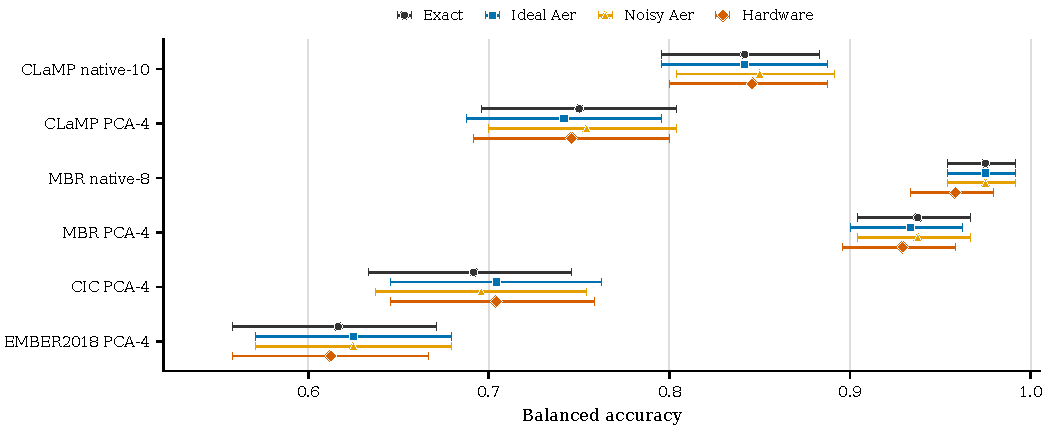
\includegraphics[width=\textwidth]{hardware_results/results/analysis/paper_figure1_execution_performance.pdf}
  \caption{Balanced accuracy across exact, ideal-Aer, noisy-Aer, and IBM hardware execution. Points are means across three held-out splits; bars are 95\% class-stratified bootstrap intervals.}
  \label{fig:execution-performance}
\end{figure*}

Kernel distortion increased with circuit width (Figure~\ref{fig:kernel-distortion}). Mean hardware relative error was approximately 0.11 for the four-qubit configurations and 0.44--0.48 for the wider circuits, while correlations with the exact kernels remained high. Across the primary hardware runs, CZ count was strongly associated with relative kernel error ($r=0.857$, Spearman $\rho=0.812$) but not with hardware-minus-exact balanced accuracy ($r=-0.032$, $\rho=-0.129$). This is a descriptive association: CZ count had only three levels, splits were clustered within configurations, and width, depth, circuit size, and CZ count increased together.

\begin{figure*}[htbp]
  \centering
  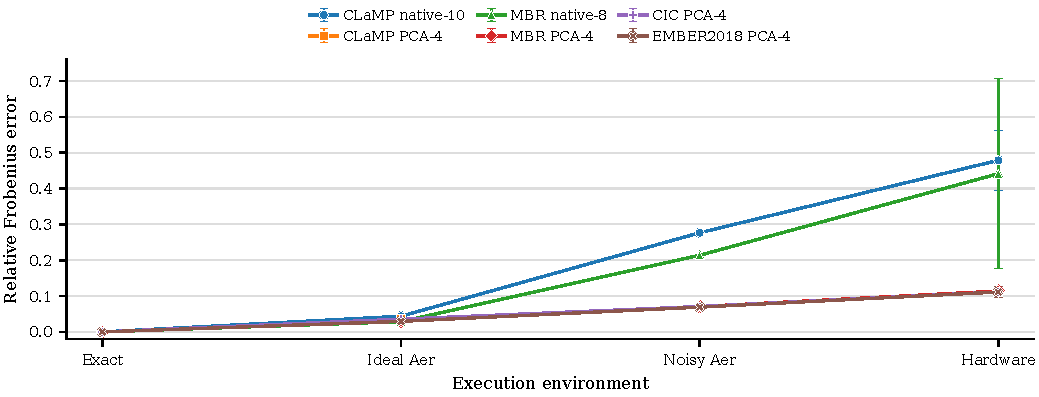
\includegraphics[width=\textwidth]{hardware_results/results/analysis/paper_figure2_kernel_distortion.pdf}
  \caption{Test-kernel relative Frobenius error against the exact statevector kernel. Markers are three-split means and error bars are split standard deviations. Exact kernels define the zero-error reference.}
  \label{fig:kernel-distortion}
\end{figure*}

PCA reduced circuit width, depth, and CZ count but produced a dataset-dependent predictive tradeoff. For CLaMP, hardware balanced accuracy decreased by 10.0 points relative to the native representation ($p=0.0179$ after Holm adjustment). The corresponding MBR decrease was 2.9 points ($p=0.458$). The matched classical comparison in Figure~\ref{fig:quantum-classical} showed no consistent quantum advantage: RBF SVC matched or exceeded hardware-quantum performance on CLaMP, CIC, and EMBER2018, whereas the quantum kernels were descriptively higher on MBR.

\begin{figure*}[htbp]
  \centering
  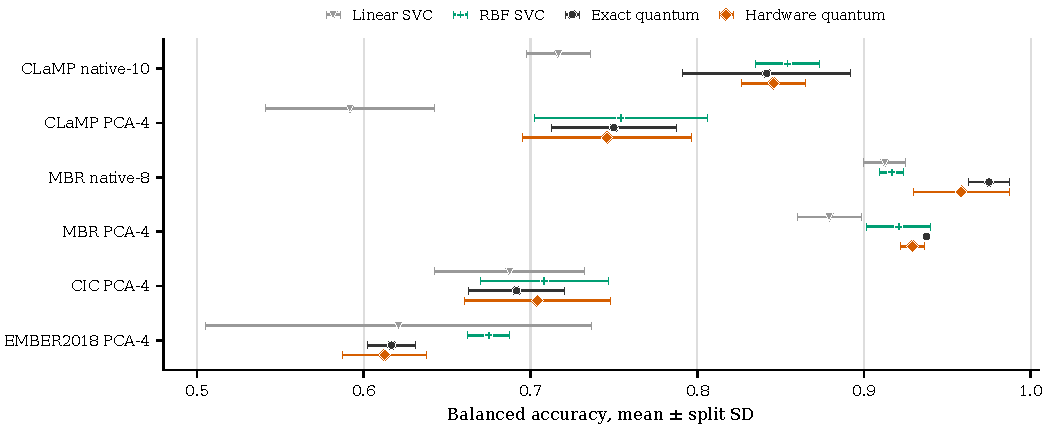
\includegraphics[width=\textwidth]{hardware_results/results/analysis/paper_figure3_quantum_classical.pdf}
  \caption{Matched linear-SVC, RBF-SVC, exact-quantum, and hardware-quantum balanced accuracy. Points are three-split means and bars are split standard deviations. Every classifier used $C=1$ without hyperparameter tuning.}
  \label{fig:quantum-classical}
\end{figure*}

The hardware experiments required approximately 103 million shots and 28,000 seconds of IBM-reported aggregate QPU usage. This aggregate usage is distinct from the estimated duration of one transpiled circuit in Table~\ref{tab:circuit-resources}.

\section{Discussion}

The principal hardware result was the stability of downstream classification despite measurable changes in the quantum kernels. Hardware execution produced substantially greater relative kernel error than exact or ideal simulation, particularly for the wider circuits, yet balanced accuracy changed by less than two percentage points. The paired tests found no significant hardware-versus-exact prediction differences after multiplicity adjustment. These findings show empirical stability for the tested samples, feature map, shot count, backend, and calibration period. They do not establish formal equivalence between exact and hardware execution.

Kernel fidelity and classification performance were not interchangeable measures in this experiment. Circuit resource requirements, represented here by CZ count, were strongly associated with kernel distortion but not with accuracy degradation. Because CZ count co-varied with circuit width, depth, and size, this analysis cannot identify CZ gates as the cause of the distortion. The hardware kernels could nevertheless differ numerically from their exact counterparts while retaining enough relative structure for the SVC to produce similar decision boundaries. This observation is specific to the tested SVC solutions; greater distortion could affect another dataset, feature map, regularization value, or set of support vectors differently.

Feature compression presented a separate tradeoff. Four-component PCA reduced qubit count, circuit depth, CZ count, and hardware-induced kernel distortion. It also removed predictive information in some configurations, with a substantial loss for CLaMP and a smaller loss for MBR. The results therefore do not support treating PCA solely as a noise-reduction step: its resource benefit must be evaluated against representation loss for each dataset.

The classical comparisons did not demonstrate a consistent accuracy advantage for the quantum kernel. RBF SVC was competitive with or better than the hardware-quantum model on CLaMP, CIC, and EMBER2018, while the quantum models were descriptively higher on MBR. These comparisons used fixed $C=1$ models without hyperparameter tuning and were intended as matched checks rather than optimized classical benchmarks. The study also did not collect comparable end-to-end wall-clock or system-level energy measurements. Accordingly, the results demonstrate neither predictive, computational, nor energy-based quantum advantage.

These findings are limited to balanced samples of 80 training and 80 test observations across three repeated holdouts, one feature-map architecture, one shot count, one backend and calibration period, and only two native-versus-PCA comparisons. Circuit width co-varied with depth, CZ count, dataset, and representation, so the resource associations are descriptive rather than causal. The classical models used fixed $C=1$ without tuning, and the study did not measure comparable wall-clock time or system-level energy use.

\section{Conclusion}

Ultimately, we have shown through this study the potential of quantum kernels, under NISQ conditions, for use in malware detection. The core principle we evaluated was whether, after applying PCA and performing feature reduction, quantum kernels could preserve learnability. The PCA-reduced representations retained predictive signal across the evaluated datasets, although predictive performance was dataset dependent. The deviation caused by device noise was small in downstream balanced accuracy compared with the numerical distortion of the kernels under the tested conditions.

In malware detection, PCA can substantially reduce the number of features without resulting in a complete loss of learning. However, PCA was not cost-free: it reduced circuit requirements and hardware kernel distortion but caused a substantial predictive loss for CLaMP and a smaller loss for MBR.

This study compared classical SVCs with exact, ideal Qiskit Aer, noisy Qiskit Aer, and IBM-hardware quantum kernels across four malware datasets. IBM hardware increasingly distorted the measured kernels as circuit resource requirements increased, but downstream balanced accuracy remained close to exact-kernel performance in all six configurations. PCA reduced circuit cost and hardware kernel distortion while causing dataset-dependent losses in predictive performance. Classical RBF models remained competitive, and the experiment did not demonstrate quantum advantage in accuracy, speed, or energy use. The results instead provide reproducible small-sample evidence that quantum-kernel malware classification can remain stable on current NISQ hardware despite substantial kernel distortion under the tested conditions.

\subsubsection{Future Work}

Future evaluations should use larger samples and further vary the tested configurations. Both the classical and quantum models may be improved through model tuning. Another useful comparison would be between this quantum support vector machine (QSVM) approach and a trainable quantum neural network (QNN) to test whether a learned representation improves predictive performance and exhibits the same sensitivity to hardware error.

Another idea that emerged from this study is to use quantum--high-performance computing (quantum-HPC) methods to evaluate quantum-kernel scalability. For example, kernel evaluation could be parallelized across groups of quantum resources based on the size of the feature space. Such methods remained outside the scope of this study.

\section{Acknowledgments}
We would like to thank the Monmouth University School of Science Summer Research Program for providing funding for this project. We also thank RPI, where this research was conducted on its on-campus IBM Quantum System One.

\bibliography{aaai24,paper_additional_references}

\end{document}
